\documentclass[12pt]{amsart}

\usepackage[margin=1in]{geometry}
\usepackage{graphicx}
\usepackage{amssymb}
\usepackage{mathtools}

\newtheorem{thm}{Theorem}[section]
\newtheorem{prop}[thm]{Proposition}
\newtheorem{lem}[thm]{Lemma}
\newtheorem{cor}[thm]{Corollary}

%\newtheorem{conj}[thm]{Conjecture} 

\theoremstyle{definition}
\newtheorem{definition}[thm]{Definition}
\newtheorem{example}[thm]{Example}

%\newtheorem{note}[thm]{Note}

\theoremstyle{remark}
\newtheorem{remark}[thm]{Remark}

\numberwithin{equation}{section}

% Macros/abbreviations

\newcommand{\N}{\mathbb{N}}
\newcommand{\R}{\mathbb{R}}
\newcommand{\Cl}{\mathcal{C}\ell}
\newcommand{\step}[1]{\noindent\textbf{Step #1}}

% Mathematical operators like sine and cosine, which are used as
% functions and have slightly different spacing when typeset

\DeclareMathOperator{\dist}{dist}

%

\begin{document}

\title{A Multi-Weighted, Multi-Constrained Path Finding Algorithm}

\author{Brad Denby}

\maketitle

\section{Introduction}

This algorithm finds the shortest satisfactory path(s) from one vertex to another in a graph with multi-weighted, directed edges subject to a multi-constraint. It briefly discusses conditions that can affect the number of calculations required before the algorithm returns a solution.

Some disciplines, including ones in the sciences, technology, engineering, mathematics, and business, use graph theory to model systems and solve problems. Biologists use graphs to model neural networks. Network engineers depend on graphs when deploying telephone and internet lines. Environmentalists employ wireless sensor networks to collect data about forest fires. Companies build graphs to analyze social networks and determine shipping routes.

Overwhelmingly, problems in graph theory revolve around finding paths from one node to another at minimal cost. Useful solutions to these problems have been known for years in simple cases, such as graphs with one or no weights associated with each edge. However, graphs in which edges have multiple weights that may be constrained by certain resource requirements are more difficult to solve. For example, connections between satellites in an orbital constellation are constrained by distance, power, and travel time for the signal.

This algorithm finds the set of multi-weighted paths that solve the multi-constrained path problem. From this set, the solution to the multi-constrained optimal path problem may be selected.

\section{Graph Theory}

\begin{definition}
An \textbf{ordered n-tuple} $(a_1, a_2, \ldots, a_n)$ is the ordered collection with $a_1$ as the first element, $a_2$ as the second element, and so on, with $a_n$ as the $n^{\text{th}}$ element. Two ordered n-tuples are equal if and only if each corresponding pair of their elements is equal, i.e. $(a_1, a_2, \ldots, a_n) = (b_1, b_2, \ldots, b_n) \iff a_1 = b_1 \land a_2 = b_2 \land \ldots \land a_n = b_n$. An \textbf{ordered pair} is a 2-tuple (Rosen 117).
\end{definition}

\begin{definition}
A \textbf{finite graph} $G = \{V,E\}$ consists of a finite set $V$ of \textbf{vertices} and a set $E$ of pairs from $V$ called \textbf{edges}. If the pair of vertices for an edge is an ordered pair, then it is said to be a \textbf{directed edge} (Rosen 589). 
\end{definition}

This algorithm focuses on finite sets $E$ of edges $e \in E$ that are directed, i.e. they are ordered pairs denoted $(a, b)$, where $a, b \in \N$ and $\{a, b\} \subseteq V$.  Here, specific vertices are each labeled by a unique natural number.

\begin{definition}
Vertex $a \in V$ is \textbf{adjacent} to vertex $b \in V$ if and only if there exists a directed edge $(a, b) \in E$ (Tucker 3).
\end{definition}

\newpage

\begin{definition}
A \textbf{walk} of \textbf{length} $k \in \N$ is an ordered $(k+1)$-tuple of vertices, i.e. $(a_1, a_2, \ldots, a_{k+1})$ with $\{a_1, a_2, \ldots, a_{k+1}\} \subseteq V$, such that the $i^\text{th}$ vertex is adjacent to the $i+1^\text{th}$ vertex, where $i \in \N : i < k+1$, i.e. $\{(a_1, a_2), (a_2, a_3), \ldots, (a_k, a_{k+1})\} \subseteq E$. A \textbf{path} is a walk in which there are exactly $k+1$ unique vertices in the ordered $(k+1)$-tuple, i.e. no vertices are revisited by the walk (Rosen 622).
\end{definition}

In other words, the term ``path" describes a specific kind of walk. Since this algorithm does not consider edge weights that reduce the overall cost of a walk, only walks that are paths need to be considered when searching for an optimal multi-constrained connection between vertices.

\begin{example}
To help demonstrate these terms, consider the pictorial representation of a graph $G=\{V,E\}$.

\begin{center}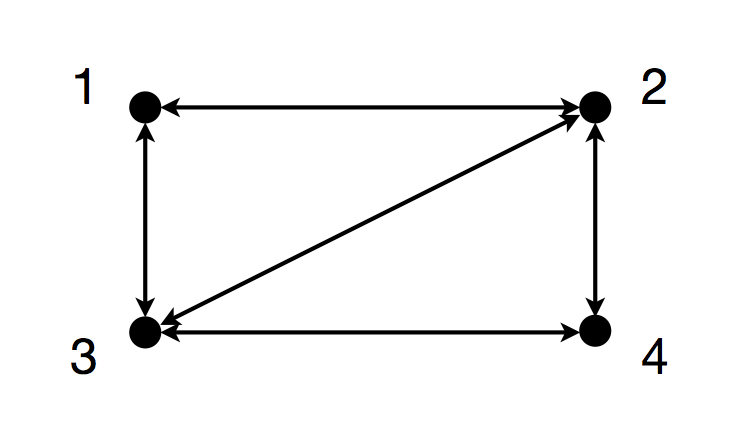
\includegraphics[width=10cm]{figure-1-2.png}\end{center}

The set $V = \{1, 2, 3, 4\}$ and the set $E = \{(1, 2), (1, 3), (2, 1), (2, 3), (2, 4), (3, 1), (3, 2), (3, 4), \allowbreak(4, 2), (4, 3)\}$, i.e. all edges $e \in E$ are directed. Vertex $1$ is adjacent to vertex $2$ and vertex $3$. There exists a path $(1, 2, 4)$ of length $2$ from vertex $1$ to vertex $4$.
\end{example}

In order to more efficiently analyze graphs, they can be translated into a form that is readily manipulated by computers. Graphs with only vertices and edges and no edge weights may be fully represented as a matrix.

\begin{definition}
Suppose the graph $G = \{V,E\}$ has $n \in \N$ vertices, and let $i \in \N$ and $j \in \N$ represent vertices so that $ i \in \N : i \le n$ and $j \in \N : j \le n$. The graph's corresponding \textbf{adjacency matrix} $\mathbf{A}$ is an $n$-by-$n$ matrix of $0$s and $1$s, where entry
$$
	a_{ij} = \left\{
		\begin{array}{ll}
			1 & i \text{ adjacent to } j \\
			0             & \text{otherwise}
		\end{array}
	\right.
$$
in row $i$ and column $j$ (Rosen 612).
\end{definition}

\newpage

\begin{example}
Consider again the pictorial representation of a graph $G = \{V,E\}$.

\begin{center}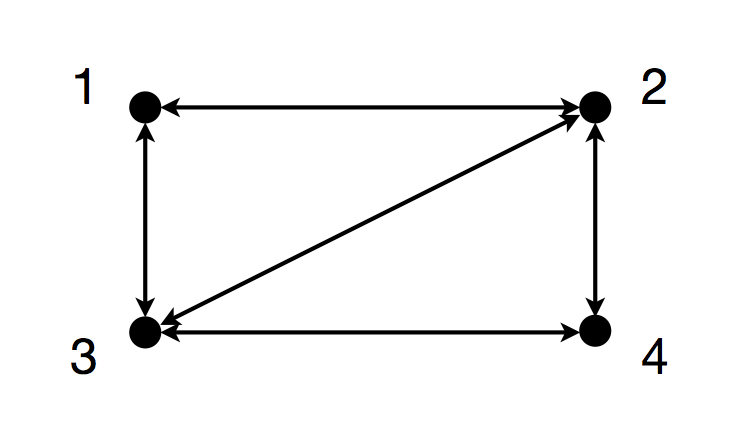
\includegraphics[width=10cm]{figure-1-2.png}\end{center}

\noindent For this graph, the corresponding adjacency matrix $\mathbf{A} = $
$
\left( \begin{array}{cccc}
0 & 1 & 1 & 0 \\
1 & 0 & 1 & 1 \\
1 & 1 & 0 & 1 \\
0 & 1 & 1 & 0 \end{array} \right)
$.
\end{example}

\begin{remark}
The example adjacency matrix is \textbf{symmetric}, i.e. $\forall i,j : a_{ij} = a_{ji}$, which is a result of the fact that, for each directed edge $(a,b) \in E$, there exists a directed edge $(b,a) \in E$. In other words, the graph could be thought of as undirected. A directed graph may have an adjacency matrix that is not symmetric (Meyer 85).
\end{remark}

Representing a graph with its adjacency matrix can be advantageous, because computers readily manipulate matrices mathematically. Proper manipulation of an adjacency matrix reveals information about walks through the graph.

For example, the adjacency matrix may be used to determine the number of walks of length $k$ from one vertex to another. First, let $\mathbf{A}$ and $\mathbf{B}$ be two $n$-by-$n$ matrices of numbers whose entries are denoted by $a_{ij}$ and $b_{ij}$ respectively, where $i \in \N : i \le n$ and $j \in \N : j \le n$. Recall that the product $\mathbf{A} \times \mathbf{B}$ is the $n$-by-$n$ matrix $\mathbf{C}$ whose entry $c_{ij}$ in row $i$ and column $j$ is given by $c_{ij} = \sum_{p=1}^n a_{ip} b_{pj}$, where $i \in \N : i \le n$ and $j \in \N : j \le n$ (Meyer 96).

\begin{thm}
Let $\mathbf{A}$ denote the adjacency matrix of a graph $G$ with $n$ vertices $a_1, a_2, \ldots, a_n$, and let $k \in \N$. Note that $\mathbf{A}^k = \mathbf{A} \times \mathbf{A} \times \ldots \times \mathbf{A}$, where $\mathbf{A}$ appears $k$ times on the right. Entry $ a_{ij} \in \mathbf{A}^k$ equals the number $m$ of walks of length $k$ in $G$ joining vertices $a_i$ and $a_j$ (Brualdi 485).
\end{thm}

\begin{proof}
by induction:

Base Case: Let $k = 1$. Then $\mathbf{A}^k = \mathbf{A}$. By definition of the adjacency matrix, if there exists a walk $(a_i, a_j)$ from vertex $a_i$ to vertex $a_j$, then $a_{ij} = 1$; otherwise, $a_{ij} = 0$. A $k+1$ item walk has a length $k$, and $G$ is restricted to graphs in which any two vertices have one or fewer edges between them. Thus, entry $a_{ij} \in \mathbf{A}^1$ equals the number of walks of length $1$ in $G$ joining vertices $a_i$ and $a_j$.

Inductive Hypothesis: Suppose that for some $k \in \N$, entry $ a_{ij} \in \mathbf{A}^k$ equals the number $m$ of walks of length $k$ in $G$ joining vertices $a_i$ and $a_j$.

Inductive Step: Note that $\mathbf{A}^{k+1} = \mathbf{A}^k \times \mathbf{A}$. From the definition of the matrix product, $c_{ij} = \sum_{p=1}^n a_{ip} b_{pj}$. Let $a_{ip} \in \mathbf{A}^k$ and $b_{pj} \in \mathbf{A}$. By the definition of adjacency matrix, if there exists a walk $(a_p, a_j)$ from vertex $a_p$ to vertex $a_j$, then $b_{pj} = 1$; otherwise, $b_{ij} = 0$. By the inductive hypothesis, $a_{ip} \in \mathbf{A}^k$ equals the number $m$ of walks of length $k$ in $G$ joining vertices $a_i$ and $a_p$.

Case 1: Suppose for some $p \in \N : p \le n$, $b_{pj} = 0$. Then there does not exist a walk $(a_p, a_j)$ from $a_p$ to $a_j$. Thus, there do not exist any walks of length $k+1$ from $a_i$ to $a_p$ and then directly from $a_p$ to $a_j$. The product $a_{ip} b_{pj} = 0$, so the sum $c_{ij} = \sum_{p=1}^n a_{ip} b_{pj}$ increases by $0$.

Case 2: Suppose for some $p \in \N : p \le n$, $b_{pj} = 1$. Then there exists a walk $(a_p, a_j)$ from $a_p$ to $a_j$. The product $a_{ip} b_{pj} = m$, so the sum $c_{ij} = \sum_{p=1}^n a_{ip} b_{pj}$ increases by $m$, which represents all walks of length $k+1$ from $a_i$ to $a_p$ (length $k$) and then directly from $a_p$ to $a_j$ (now length $k+1$).

Therefore, by induction, entry $a_{ij} \in \mathbf{A}^k$ equals the number $m$ of walks of length $k$ in $G$ joining vertices $a_i$ and $a_j$.
\end{proof}

As defined, an adjacency matrix enables some analysis of graphs with one or zero edges between any given two vertices. However, some graphs utilize more than one edge between any given two vertices. Additionally, graphs modeling complex systems often employ more than just vertices and edges to encode information.

\begin{definition}
A graph $G = \{V,E\}$ for which each edge $e \in E$ corresponds to a \textbf{weight} $w \in \R$ is a \textbf{weighted graph}. Edges of such a graph are called \textbf{weighted edges}. In a weighted graph, the length $k$ of a walk equals the sum of all of the weights corresponding to the walk's edges. Note that this sum can be according to a general addition operation, however it may be defined (Rosen 647).
\end{definition}

\begin{remark}
Most generally, an edge weight could be ``negative," e.g. a walk $(a_1,a_2, \ldots, a_n)$ could have a length $k_1$ greater than the length $k_2$ of a walk $(a_1,a_2, \ldots, a_n, a_{n+1})$ if the weight of the edge $(a_n, a_{n+1})$ is less than zero. This algorithm only considers nonnegative weights.
\end{remark}

\begin{example}
In this pictorial representation, the graph $G = \{V,E\}$ is a weighted graph.

\begin{center}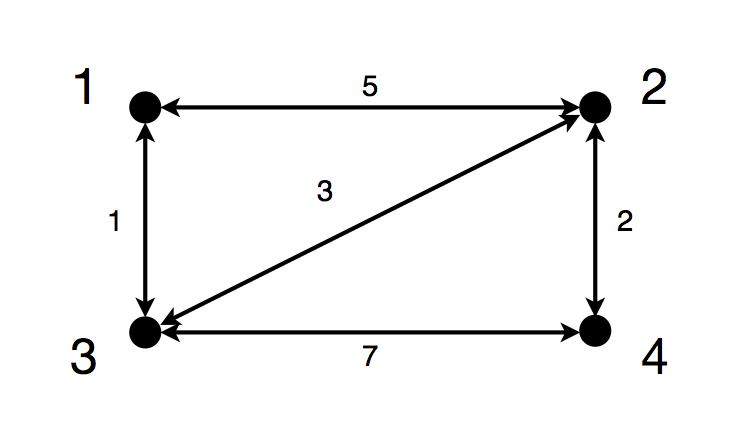
\includegraphics[width=10cm]{figure-3.png}\end{center}

The edge $(1,2)$ has length $5$, the edge $(2,4)$ has length $2$, and the path $(4,2,1)$ has length $2+5 = 7$.
\end{example}

As it is currently defined, the adjacency matrix does not encode edge weight information. Since edge weights affect the length $k$ of walks, the graph analysis technique using the previously described adjacency matrix cannot be applied to weighted graphs.

Many efficient algorithms exist for analyzing weighted graphs. However, many of these algorithms focus on graphs in which one weight corresponds to each edge. Fewer efficient options exist for analyzing graphs with more than one weight per edge.

\begin{definition}
A graph $G = \{V,E\}$ for which each edge $e \in E$ corresponds to a \textbf{multi-weight} vector $\vec{w} \in \R^d$ of dimension $d$ is a \textbf{multi-weighted graph}. An edge of such a graph is called \textbf{multi-weighted edge}. In a multi-weighted graph, the multi-weight $\vec{k} \in \R^d$ of a walk equals the vector sum of all of the multi-weights corresponding to the walk's edges (Kahng 216).
\end{definition}

\begin{example}
Consider the following multi-weighted graph $G = \{V,E\}$.

\begin{center}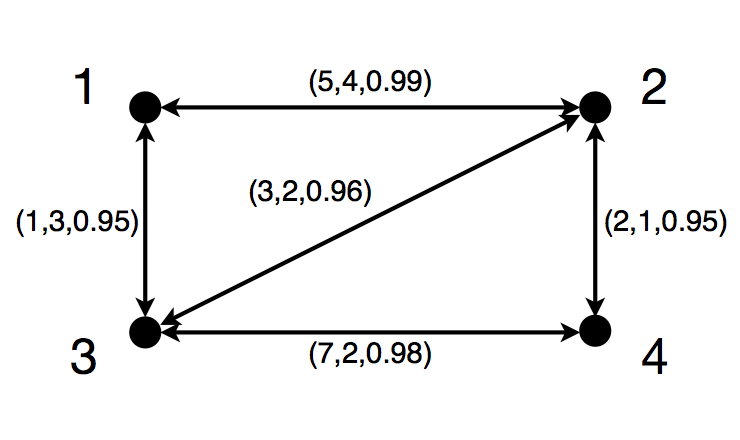
\includegraphics[width=10cm]{figure-4-5-6.png}\end{center}

The edge $(1,2)$ has a multi-weight $(5, 4, 0.99)$, and the edge $(2,4)$ has a multi-weight $(2,1,0.95)$. Under the usual definition of addition, the path $(4,2,1)$ has a multi-weight $(2+5, 1+4, 0.95+0.99) = (7, 5, 1.94)$. 
\end{example}

In the example, the total path cost is given according to the ``usual" definition of addition. However, edge costs need not sum in the ``usual" fashion. In fact, it is often the case that edge costs interact in ways that are not additive. For example, a graph being used to model a network might keep track of data flow, disallowing packets of data greater than 512 kb from being transferred between nodes. A graph that models a neural network may keep track of the probability that one neuron will trigger another, and interactions that fall below a certain probability are discounted.

Accounting for the possibility of a mix of weights with different behaviors requires a different definition for the vector sum.

\begin{definition}
Let the multi-weight $\vec{w} \in \R^d$. Then there are at least $1$ and at most $d$ different \textbf{types} of weights occupying the coordinates of $\vec{w}$: $t_1$ weights of type $1$, $t_2$ weights of type $2$, and so on up to $t_n$ weights of type $n$ where $n \le d$ and $\sum_{i=1}^n t_i = d$. All weights of type $1$ occupy the first $t_1$ coordinates of $\vec{w}$, all weights of type $2$ occupy the next $t_2$ coordinates of $\vec{w}$, and so on, so that all weights of type $n$ occupy the last $t_n$ coordinates of $\vec{w}$. The vector sum between two multi-weights is defined to be the component-wise addition of corresponding coordinates using that coordinate's definition of addition. The first $t_1$ weights add according to type $1$ addition, the next $t_2$ weights add according to type $2$ addition, and so on. Addition $\boxplus$ between two multi-weight vectors $\vec{w_1}, \vec{w_2}$ is defined only if the weight types match for each coordinate.
\end{definition}

Generally, two weights $w_1$, $w_2$ of matching type $i$ located in corresponding coordinates of two multi-weights being added  interact under a general operation $\ast$, i.e. $w_1 \ast w_2$.  The following definitions introduce three specific types of weights, replacing the general operator $\ast$ with the specific operators $+$, $\vee$, and $\cdot$.

\begin{definition}
An \textbf{additive weight} $w \in \R_{\ge 0}$ sums as usual, i.e. for $w_1 \in \R_{\ge 0}$ and $w_2 \in \R_{\ge 0}$ the sum $w_1 + w_2$ acts as expected for real numbers.
\end{definition}

\begin{definition}
For a \textbf{maximal weight} $w \in \R_{\ge 0}$, the sum outputs the maximum of the two inputs. Namely, $w_1 \vee w_2 = \max\{w_1,w_2\}$.
\end{definition}

\begin{definition}
\textbf{Multiplicative weights} $w \in [0,1] \subset \R$ multiply under the addition operator. So the sum $w_1 \cdot w_2$ outputs the product between the two real numbers.
\end{definition}

Note that $0 \in \R_{\ge 0}$ acts as an identity with $+$ for the additive weights, $0 \in \R_{\ge 0}$ acts as an identity with $\vee$ for the maximal weights, and $1 \in [0,1] \subset \R$ acts as an identity with $\cdot$ for the multiplicative weights.

Using these three types of weights, reconsider the multi-weighted graph where each multi-weight $\vec{w}$ is three-dimensional, and where the first weight is now an additive weight, the second weight is now a maximal weight, and the third weight is a now multiplicative weight. For the two weights $(w_1, w_2, w_3)$ and $(w_4, w_5, w_6)$, the sum $(w_1, w_2, w_3) \boxplus (w_4, w_5, w_6) = (w_1 + w_4, w_2 \vee w_5, w_3 \cdot w_6)$.

\begin{remark}
A multi-weight can be conceptualized as the direct product between weight type semigroups. Let the type $1$ semigroup $T_1 = (\R_{\ge 0}, +)$, the type $2$ semigroup $T_2 = (\R_{\ge 0}, \vee)$, and the type $3$ semigroup $T_3 = ([0,1] \subset \R, \cdot)$. Then the multi-weights belong to the semigroup $W = T_1 \otimes T_2 \otimes T_3$ with the operation $\boxplus$. Since the additive, maximal, and multiplicative semigroups each have an identity element under their respective binary operation, these semigroups are also monoids.
\end{remark}

\begin{example} Consider the multi-weighted graph $G = \{V,E\}$.

\begin{center}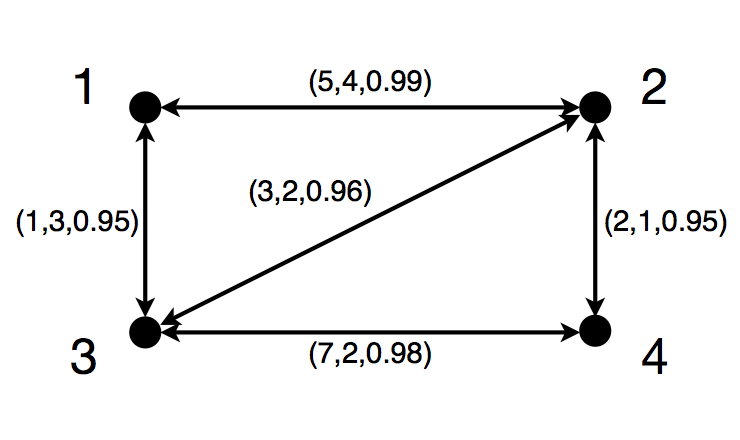
\includegraphics[width=10cm]{figure-4-5-6.png}\end{center}

The edge $(1,2)$ has a multi-weight $(5, 4, 0.99)$ and the edge $(2,4)$ has a multi-weight $(2,1,0.95)$. For these multi-weights, the first coordinate is additive, the second coordinate is maximal, and the third coordinate is multiplicative. Under the multi-weight vector sum definition of addition, the path $(4,2,1)$ has a multi-weight $(2+5, \max\{1,4\}, 0.95 \cdot 0.99) = (7, 4, 0.9405)$.
\end{example}

While these multi-weight vectors composed of different types of weights adequately describe graphs with edge weights that interact with different behaviors, they do not yet account for the previously proposed scenarios. For example, multi-weight vectors would track the maximum size of a packet between network nodes or the probability of one neuron triggering another. However, walks requiring packets greater than 512 kb and walks with a probability below the set threshold for triggering a neuron are not differentiated from acceptable walks. Fully modeling these scenarios requires the introduction of constraints.

\begin{definition}
A \textbf{constraint} $s$ corresponds to a weight $w \in W$, partitioning the set of weights $W$ into a subset $W_s \subseteq W$ of weights that satisfy the constraint and a subset $W_u \subseteq W$ of weights that do not satisfy the constraint, where $W_s \cap W_u = \emptyset$ (Kahng 216).
\end{definition}

The rule for partitioning weights into satisfying and unsatisfying sets depends on the type of weight. As examples, consider the following constraints for additive, maximal, and multiplicative types of weights.

\begin{definition}
An additive weight $w_1 \in \R_{\ge 0}$ satisfies the constraint $s_+ \in \R_{\ge 0} \cup \{\infty\}$ if and only if $w < s_+$. A maximal weight $w_2 \in \R_{\ge 0}$ satisfies the constraint $s_{\vee} \in \R_{\ge 0}$ if and only if $w < s_{\vee}$. A multiplicative weight $w_3 \in [0,1] \subset \R$ satisfies the constraint $s_{\cdot} \in [0,1] \subset \R$ if and only if $w > s_{\cdot}$.
\end{definition}

Just as a constraint corresponds to a weight, a multi-constraint corresponds to a multi-weight.

\begin{definition}
A \textbf{multi-constraint} vector $\vec{s} \in \R^d$ of dimension $d$ corresponds to a set $W$ of all multi-weight vectors possible for a graph $G$, with each multi-weight $\vec{w} \in \R^d$. A multi-weight vector satisfies the multi-constraint only if each weight $w$ in $\vec{w}$ satisfies the the constraint $s$ in the corresponding coordinate of $\vec{s}$ (Kahng 216).
\end{definition}

\begin{example}
Return again to the multi-weighted graph $G = \{V,E\}$. This time, the graph $G$ is constrained by the multi-constraint $(7,4,0.85)$.

\begin{center}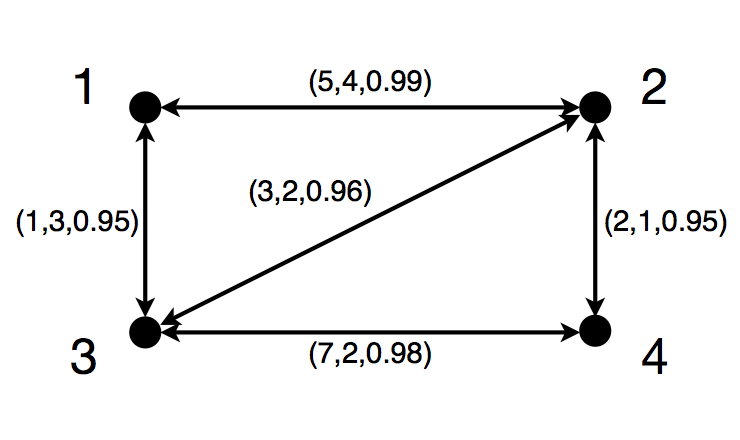
\includegraphics[width=10cm]{figure-4-5-6.png}\end{center}

The multi-weight $(5, 4, 0.99)$ of edge $(1,2)$ does not satisfy the multi-constraint, since $4 \not< 4$. The edge $(2,4)$ does satisfy the multi-constraint with a multi-weight $(2,1,0.95)$. Using addition as defined above, the path $(4,2,1)$ has a multi-weight $(7, 4, 0.9405)$, which does not satisfy the multi-constraint since $4 \not< 4$.
\end{example}

These definitions provide a framework in which to begin considering the fundamental problems with which this project is concerned.

\begin{definition}
The \textbf{multi-constrained path problem} seeks to find paths between any two vertices in a graph $G$ such that the multi-weight $\vec{w}$ of that path satisfies the corresponding multi-constraint vector (Schott). % also Djikstra's two problems in graphs
\end{definition}

Finding the set of paths satisfying the multi-constraint is usually not the only goal. More often, the problem is finding the \textit{optimal} path between two vertices.

\begin{definition}
Let $P$ be the set of paths between two given vertices in a graph $G$ whose multi-weights satisfy the multi-constraint, i.e. the solution to the multi-constrained path problem. The \textbf{multi-constrained optimal path problem} seeks to find the optimal path $p \in P$ (Schott).
\end{definition}

The solution to these problems benefits from some abstract algebra techniques in addition to the preceding framework from graph theory. Specifically, it would be advantageous if, rather than simply partitioning the walks into satisfactory and unsatisfactory sets, the unsatisfactory sets could be algebraically eliminated.

\section{Abstract Algebra}

\begin{definition}
A \textbf{semigroup} $(K, \ast)$ is a set $K$ with an associative binary operation $\ast$, i.e. $\forall a, b, c \in K : (a \ast b) \ast c = a \ast (b \ast c)$. A \textbf{monoid} is a semigroup with an identity element $e \in K$ for the binary operation $\ast$, i.e. $\forall a \in K : e \ast a = a \ast e = a$ (Fraleigh 42).
\end{definition}

\begin{definition}
A \textbf{hemiring} $(K, +, \ast)$ is a nonempty set $K$ with addition and multiplication operations such that
\begin{enumerate}
\item $(K, +)$ is a commutative monoid, i.e. $\forall a, b \in K : a + b = b + a$ with an identity element $0$,
\item $(K, \ast)$ is a semigroup,
\item Multiplication distributes over addition from either side, i.e. $\forall a, b, c \in K : a \ast (b + c) = (a \ast b) + (a \ast c)$ and $(a + b) \ast c = (a \ast c) + (b \ast c)$,
\item  $\forall a \in K : 0 \ast a = a \ast 0 = 0$ (Golan 1).
\end{enumerate}
\end{definition}

\begin{example}
Elaborating on the ideas of \textit{Remark 2.19}, the additive weight type may be expanded to a hemiring. For the additive weight hemiring $(\R_{\ge 0}, +, \ast)$, $(\R_{\ge 0}, +)$ is a commutative monoid with an additive identity $0$, $(\R_{\ge 0}, \ast)$ is a semigroup, multiplication distributes over addition from either side, and $\forall w \in \R_{\ge 0} : 0 \ast w = w \ast 0 = 0$.
\end{example}

Note that while this example does present the additive weight type as a hemiring, a different hemiring (a ``cost hemiring") will be introduced in order to prune weights that do not satisfy their constraints.

\section{Eliminating Walks That Are Not Paths}

\begin{definition}
Consider a graph $G = \{V,E\}$, and let $P$ be a set such that every vertex $v \in V$ corresponds to exactly one element $p_{(v)} \in P$. Define the \textbf{path hemiring} $(P,+,\cdot)$ such that $(P,+)$ is a commutative monoid with an identity $0$, $(P,\cdot)$ is a semigroup, multiplication distributes over addition from either side, and $\forall p \in P : 0 \cdot p = p \cdot 0 = 0$. Define the binary operation $\cdot$ as follows:
$$
	p_{u} \cdot p_{v}  = \left\{
		\begin{array}{ll}
			p_{u.v} & u.v \text{ is a path in } G \\
			0             & \text{otherwise}
		\end{array}
	\right.
$$
where $u$ is an ordered m-tuple $(u_1, u_2, \ldots, u_m)$, $v$ is an ordered n-tuple $(v_1, v_2, \ldots, v_n)$, the set $\{u_1, u_2, \ldots, u_m, v_1, v_2, \ldots, v_n\} \subseteq V$, and `$.$' indicates concatenation with the requirement that $u_m \in V$ is adjacent to $v_1 \in V$.
\end{definition}

\begin{example}
Consider the multi-weighted graph $G = \{V,E\}$, where the vertices are labeled with elements from the path hemiring.

\begin{center}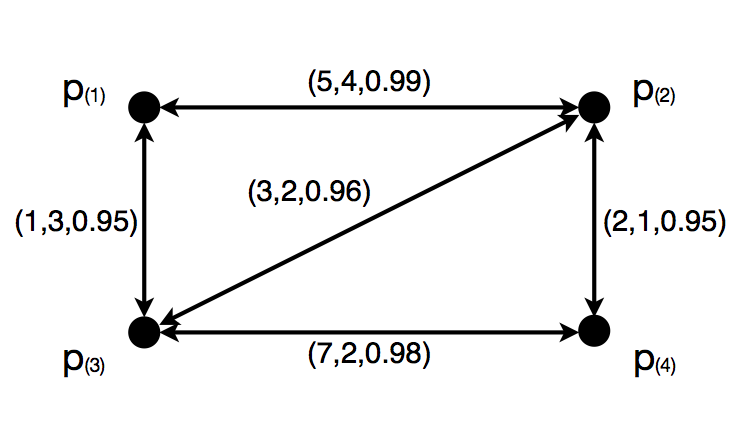
\includegraphics[width=10cm]{figure-7.png}\end{center}

The path from $p_{(1)}$ to $p_{(4)}$ via $p_{(2)}$ is obtained by $p_{(1)}p_{(2)}p_{(4)} = p_{(1,2,4)}$, a walk that revisits a vertex $p_{(3)}p_{(2)}p_{(4)}p_{(3)} = 0$, and multiplying the elements $p_{(1)}$ and $p_{(4)}$ gives a result of $0$ because these vertices are not adjacent.
\end{example}

\section{Eliminating Unsatisfying Weights}

\begin{definition}
Consider a multi-weighted graph $G = \{V,E\}$, and let $C$ be a set such that every edge $e \in E$ corresponds to exactly one element $c^{\vec{w}} \in C$, where $\vec{w}$ is the multi-weight associated with the edge $e$. Define the \textbf{cost hemiring} $(C, +, \cdot)$ such that $(C, +)$ is a commutative monoid with an identity $0$, $(C, \cdot)$ is a semigroup, multiplication distributes over addition from either side, and $\forall c \in C : 0 \cdot c = c \cdot 0 = 0$. Define the binary operation $\cdot$ as follows:
$$
	c^{\vec{w_1}} \cdot c^{\vec{w_2}}  = \left\{
		\begin{array}{ll}
			c^{\vec{w_1} \boxplus \vec{w_2}} & \vec{w_1} \boxplus \vec{w_2} \text{ satisfies the multi-constraint } \vec{s} \\
			0             & \text{otherwise}
		\end{array}
	\right.
$$
An element $c^{\vec{w}} \in C$ is referred to as a \textbf{cost}.
\end{definition}

\begin{example}
Consider the graph $G = \{V, E\}$, where each multi-weight label is replaced with an element from the cost hemiring. The multi-constraint is $(7, 4, 0.85)$, and the multi-weight coordinates contain additive, maximal, and multiplicative weight types respectively.

\begin{center}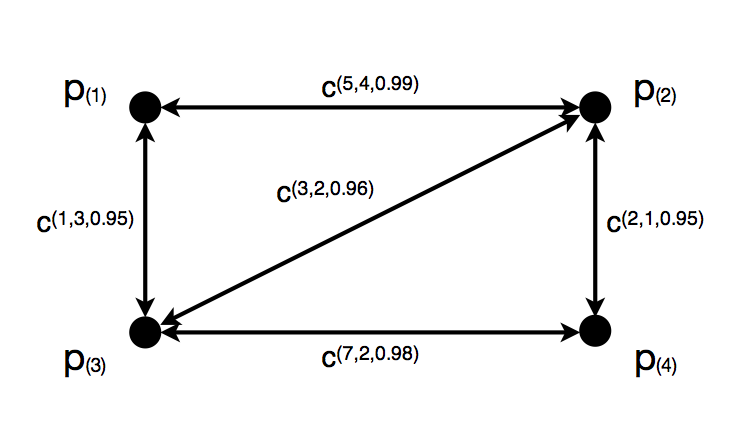
\includegraphics[width=10cm]{figure-8-plus.png}\end{center}

The product $c^{(1,3,0.95)} \cdot c^{(7,2,0.98)} = c^{(1,3,0.95) \boxplus (7,2,0.98)} = c^{(8,3,0.931)} = 0$, since the multi-weight $(8,3,0.931)$ does not satisfy the multi-constraint $(7, 4, 0.85)$. The product $c^{(1,3,0.95)} \cdot c^{(3,2,0.96)} = c^{(1,3,0.95) \boxplus (3,2,0.96)} = c^{(4,3,0.912)}$.
\end{example}

\section{The Cost-Path Matrix}

By considering the direct product between the path hemiring and the cost hemiring, all walks that do not solve the multi-constrained path problem are eliminated, and the number of solution candidates for the multi-constrained optimal path problem is reduced.

\begin{example}
Let $v$ represent a path in the graph $G = \{V,E\}$, let $\vec{w}$ represent the multi-weight with multi-constraint $\vec{s}$ that corresponds to $v$, let $p_v$ be the element of the path hemiring that corresponds to $v$, and let $c^{\vec{w}}$ be the element of the cost hemiring that corresponds to $\vec{w}$. Using the definitions for the path hemiring and the cost hemiring, the direct product
$$
	c^{\vec{w}} \otimes p_v = \left\{
		\begin{array}{ll}
			0 & c^{\vec{w}} = 0 \text{ or } v_p = 0 \\
			c^{\vec{w}} p_v & \text{otherwise}
		\end{array}
	\right.
$$
In other words, paths with unsatisfying multi-weights and walks that are not paths are sent to $0$.
\end{example}

\begin{remark}
Sending an element $c^{\vec{w}} p_v$ to $0$ in the case that $\vec{w}$ does not correspond to the path $v$, while not essential due to the deliberate design of the algorithm, makes for a more robust algebra.
\end{remark}

The resulting cost-path hemiring can be used to list cost-paths with addition:

\begin{example}
Let $G = \{V,E\}$ be a graph, and suppose there exist exactly two paths $(i, r_1, j)$ and $(i, r_2, j)$ of length $2$ from vertex $i \in V$ to vertex $j \in V$ in $G$. Suppose that the multi-weight $\vec{w}_1$ corresponds to the path $(i, r_1, j)$, and the multi-weight $\vec{w}_2$ corresponds to the path $(i, r_2, j)$. Then the cost-path element $c^{\vec{w}_1} p_{(i, r_1, j)}$ represents the path $(i, r_1, j)$ with multi-weight $\vec{w}_1$, the cost-path element $c^{\vec{w}_2} p_{(i, r_2, j)}$ represents the path $(i, r_2, j)$ with multi-weight $\vec{w}_2$, and the expression $c^{\vec{w}_1} p_{(i, r_1, j)} + c^{\vec{w}_2} p_{(i, r_2, j)}$ lists all length $2$ paths with their corresponding multi-weight from vertex $i$ to vertex $j$ in $G$.
\end{example}

and to extend existing cost-paths with multiplication:

\begin{example}
Let $G = \{V,E\}$ be a graph, and let $c^{\vec{w_1}} p_{v_1}$ and $c^{\vec{w_2}} p_{v_2}$ correspond to two multi-constrained, multi-weighted paths of $G$. According to the definitions,
$$
	c^{\vec{w_1}} p_{v_1} \cdot  c^{\vec{w_2}} p_{v_2} = \left\{
		\begin{array}{ll}
			c^{\vec{w_1}\boxplus\vec{w_2}} p_{v_1.v_2} & \vec{w_1} \boxplus \vec{w_2} \text{ satisfies the multi-constraint } \vec{s} \\
			   & \text{and } v_1.v_2 \text{ is a path in } G \\
			0 & \text{otherwise}
		\end{array}
	\right.
$$
\end{example}

The multi-constrained path problem may be restated using these ideas. Consider a graph $G = \{V,E\}$. Given a start vertex $i \in V$ and an end vertex $j \in V$, the solution to the multi-constrained path problem may be expressed as a set $S$ of nonzero elements $c^{\vec{w}} p_{(i,r,\ldots,j)}$ from a cost-path hemiring, where the ordered tuples $(i,r,\ldots,j)$ of varying lengths represent all paths in $G$ that correspond to a satisfactory multi-weight $\vec{w}$ under a multi-constraint $\vec{s}$.

The solution to the multi-constrained optimal path problem is an element $c^{\vec{w}} p_{(i,r,\ldots,j)} \in S$ that corresponds to the optimal path $(i,r,\ldots,j)$ from $i$ to $j$ with a multi-weight $\vec{w}$.

Together, these ideas suggest an alternative to the adjacency matrix for graphs that employ more than just vertices and edges to model systems.

\begin{definition}
A \textbf{cost-path matrix} is similar in spirit to the adjacency matrix defined previously, with some additional functionality. Suppose the graph $G = \{V,E\}$ has $n \in \N$ vertices, and let $i, j \in V$, where  $i \in \N : i \le n$ and $j \in \N : j \le n$. The graph's corresponding cost-path matrix $\mathbf{M}$ is an $n$-by-$n$ matrix whose entry $m_{ij}$ in row $i$ and column $j$ is given by
$$
	m_{ij} = \left\{
		\begin{array}{ll}
			c^{\vec{w}} p_{(j)} & i \text{ is adjacent to } j \\
			0             & \text{otherwise}
		\end{array}
	\right.
$$
if, for all vertices $v_1, v_2 \in V$, there exists at most one edge from $v_1$ to $v_2$. In this case, $c^{\vec{w}}$ is the cost such that the multi-weight $\vec{w}$ corresponds to the only edge from vertex $i$ to vertex $j$ with multi-constraint $\vec{s}$ (Staples).\\
In the more general case where, for all vertices $v_1, v_2 \in V$, there exists any number $f \in \N$ of edges from $v_1$ to $v_2$,
$$
	m_{ij} = \left\{
		\begin{array}{ll}
			c^{\vec{w}_1} p_{(j)} + c^{\vec{w}_2} p_{(j)} + \ldots + c^{\vec{w}_f} p_{(j)} & i \text{ is adjacent to } j \text{ with multi-weight } \vec{w}_1 \text{,} \\
			& i \text{ is adjacent to } j \text{ with multi-weight } \vec{w}_2 \text{,} \\
			& \ldots \text{, and} \\
			& i \text{ is adjacent to } j \text{ with multi-weight } \vec{w}_f \\
			0             & \text{otherwise}
		\end{array}
	\right.
$$
where each cost $c^{\vec{w}_h}$ with $h \in \N : h \le f$ corresponds the the multi-weight $\vec{w}_h$ from vertex $i$ to vertex $j$ with multi-constraint $\vec{s}$.\\
Written more concisely:
$$
	m_{ij} = \left\{
		\begin{array}{ll}
			p_{(j)} \displaystyle\sum_{h=1}^f c^{\vec{w}_h} & i \text{ is adjacent to } j \text{ with multi-weights } \vec{w}_1, \vec{w}_2, \ldots, \vec{w}_f \\
			0             & \text{otherwise}
		\end{array}
	\right.
$$
\end{definition}

\begin{example}
Consider the graph $G = \{V, E\}$, with each vertex labeled by an element of the path hemiring, each edge labeled by an element from the cost hemiring, and with a multi-constraint $(7, 4, 0.85)$ of additive, maximal, and multiplicative weight types, respectively.

\begin{center}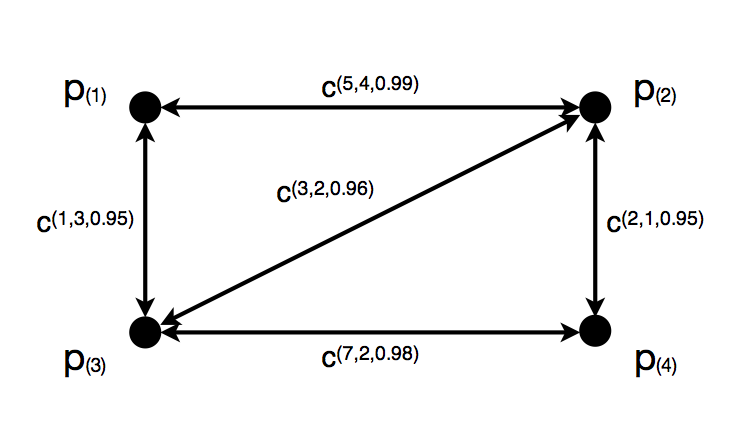
\includegraphics[width=10cm]{figure-8-plus.png}\end{center}

\noindent For this graph, the corresponding cost-path matrix
$$
\mathbf{M} = 
\left( \begin{array}{cccc}
0 & c^{(5,4,0.99)} p_{(2)} & c^{(1,3,0.95)} p_{(3)} & 0 \\
c^{(5,4,0.99)} p_{(1)} & 0 & c^{(3,2,0.96)} p_{(3)} & c^{(2,1,0.95)} p_{(4)} \\
c^{(1,3,0.95)} p_{(1)} & c^{(3,2,0.96)} p_{(2)} & 0 & c^{(7,2,0.98)} p_{(4)} \\
0 & c^{(2,1,0.95)} p_{(2)} & c^{(7,2,0.98)} p_{(3)} & 0 \end{array} \right)
$$
\end{example}

\begin{remark}
Notice that, despite the fact that the graph has the same structure as the graph in \textit{Example 2.7} with the adjacency matrix, this cost-path matrix is not symmetric, while the adjacency matrix is symmetric. The lack of symmetry is due to the fact that the elements of the path hemiring distinguish the vertices.
\end{remark}

Consider a graph $G = \{V,E\}$ with $n \in \N$ vertices and the corresponding $n$-by-$n$ cost-path matrix $\mathbf{M}$. Let the diagonal matrix
$$
\mathbf{D} =
\left( \begin{array}{cccc}
p_{(1)} & 0 & \cdots & 0 \\
0 & p_{(2)} & \cdots & 0 \\
\vdots & \vdots & \ddots & \vdots \\
0 & 0 & \cdots & p_{(n)} \end{array} \right)
$$
so that, for each element $d_{ij}$ in row $i$ and column $j$ of the matrix $\mathbf{D}$,
$$
	d_{ij} = \left\{
		\begin{array}{ll}
			p_{(i)} & i = j \\
			0          & \text{otherwise}
		\end{array}
	\right.
$$
where $i \in \N : i \le n$ and $j \in \N : j \le n$.

\begin{prop}
Left-multiplying an $n$-by-$n$ cost-path matrix $\mathbf{M}$ by the $n$-by-$n$ diagonal matrix $\mathbf{D}$ results in an $n$-by-$n$ matrix $\mathbf{P}_1 = \mathbf{D}\mathbf{M}$ whose entry $\prescript{1}{}{p_{ij}}$ in row $i$ and column $j$ lists exactly all satisfactory paths of length $1$ in $G$ from vertex $i$ to vertex $j$ along with the corresponding multi-weight for each of these paths.
\end{prop}

\begin{proof}
By the definition of matrix multiplication, each entry $\prescript{1}{}{p_{ij}} \in \mathbf{P}_1$ is given by $\prescript{1}{}{p_{ij}} = \sum_{r=1}^n d_{ir} m_{rj} = d_{i1}m_{1j} + d_{i2}m_{2j} + \ldots + d_{in}m_{nj} = d_{ii}m_{ij} = p_{(i)} m_{ij} = p_{(i)} \cdot p_{(j)} \sum_{h=1}^f c^{\vec{w}_h}$.

If $i$ is adjacent to $j$ with satisfactory multi-weights $\vec{w}_1, \vec{w}_2, \ldots, \vec{w}_f$ (case 1), then $\prescript{1}{}{p_{ij}} = p_{(i,j)} \sum_{h=1}^f c^{\vec{w}_h}$, where the costs $\sum_{h=1}^f c^{\vec{w}_h}$ list the multi-weights corresponding to the edges between vertex $i$ and vertex $j$ as required by the definition of the cost-path matrix.

Otherwise (case 2), $\prescript{1}{}{p_{ij}} = 0$, indicating zero satisfactory paths of length $1$ in $G$ from vertex $i$ to vertex $j$.

Note that, for all other entries in $\mathbf{P}_1$, either the start vertex is not $i$ or the end vertex is not $j$, which means that no entry in $\mathbf{P}_1$ other than $\prescript{1}{}{p_{ij}}$ describes any paths from vertex $i$ to vertex $j$.

Further, suppose there exists a satisfactory path of length $1$ in $G$ from vertex $i$ to vertex $j$ that is not listed in entry $\prescript{1}{}{p_{ij}}$ (i.e. it does not appear in $\mathbf{P}_1$). Since the path from $i$ to $j$ is of length $1$, then vertex $i$ is adjacent to vertex $j$. As a result, the cost-path element $c^{\vec{w}} p_{(j)}$ corresponding to this edge is listed in entry $m_{ij}$ of the cost-path matrix. Since this element is accounted for in $m_{ij}$, then this satisfactory path of length $1$ is accounted for in $\prescript{1}{}{p_{ij}}$, a contradiction of the supposition that this path is not listed in $\prescript{1}{}{p_{ij}}$. Thus, if there exists a satisfactory path of length $1$ in $G$ from vertex $i$ to vertex $j$, then it is listed in entry $\prescript{1}{}{p_{ij}}$.

Therefore, entry $\prescript{1}{}{p_{ij}}$ in row $i$ and column $j$ of $\mathbf{P}_1$ lists exactly all satisfactory paths of length $1$ in $G$ from vertex $i$ to vertex $j$ along with the corresponding multi-weight for each of these paths.
\end{proof}

\begin{example}
Consider the cost-path matrix $\mathbf{M}$ from \textit{Example 6.6} and the product $\mathbf{D}\mathbf{M}$.
$$
\begin{pmatrix}
p_{(1)} & 0 & 0 & 0 \\
0 & p_{(2)} & 0 & 0 \\
0 & 0 & p_{(3)} & 0 \\
0 & 0 & 0 & p_{(n)} \end{pmatrix} \begin{pmatrix}
0 & c^{(5,4,0.99)} p_{(2)} & c^{(1,3,0.95)} p_{(3)} & 0 \\
c^{(5,4,0.99)} p_{(1)} & 0 & c^{(3,2,0.96)} p_{(3)} & c^{(2,1,0.95)} p_{(4)} \\
c^{(1,3,0.95)} p_{(1)} & c^{(3,2,0.96)} p_{(2)} & 0 & c^{(7,2,0.98)} p_{(4)} \\
0 & c^{(2,1,0.95)} p_{(2)} & c^{(7,2,0.98)} p_{(3)} & 0 \end{pmatrix}
$$
The result of the product is the matrix $\mathbf{P}_1$.
$$
\mathbf{P}_1 = \begin{pmatrix}
0 & c^{(5,4,0.99)} p_{(1,2)} & c^{(1,3,0.95)} p_{(1,3)} & 0 \\
c^{(5,4,0.99)} p_{(2,1)} & 0 & c^{(3,2,0.96)} p_{(2,3)} & c^{(2,1,0.95)} p_{(2,4)} \\
c^{(1,3,0.95)} p_{(3,1)} & c^{(3,2,0.96)} p_{(3,2)} & 0 & c^{(7,2,0.98)} p_{(3,4)} \\
0 & c^{(2,1,0.95)} p_{(4,2)} & c^{(7,2,0.98)} p_{(4,3)} & 0 \end{pmatrix}
$$
Consider the corresponding graph $G = \{V,E\}$.

\begin{center}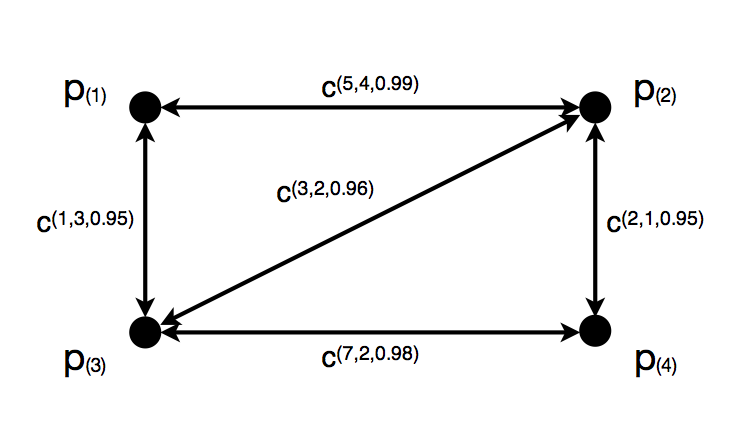
\includegraphics[width=10cm]{figure-8-plus.png}\end{center}

\noindent Entry $\prescript{1}{}{p_{12}} \in \mathbf{P}_1$ describes all multi-weighted paths of length $1$ from vertex $1$ to vertex $2$, entry $\prescript{1}{}{p_{23}} \in \mathbf{P}_1$ describes all multi-weighted paths of length $1$ from vertex $2$ to vertex $3$, and so on.
\end{example}

\begin{prop}
Left-multiplying the $n$-by-$n$ cost-path matrix $\mathbf{M}$ by its corresponding $n$-by-$n$ matrix $\mathbf{P}_1$ results in an $n$-by-$n$ matrix $\mathbf{P}_2 = \mathbf{P}_1 \mathbf{M}$ whose entry $\prescript{2}{}{p_{ij}}$ in row $i$ and column $j$ lists exactly all satisfactory paths of length $2$ in $G$ from vertex $i$ to vertex $j$ along with the corresponding multi-weight for each of these paths.
\end{prop}

\begin{proof}
Note that, for some start vertex $i$ and end vertex $j$ in $G$, all paths of length $2$ are described by a path hemiring element $p_{(i,r,j)}$, where $r \in \N : r \le n$, i.e. there are no paths from vertex $i$ to vertex $j$ in $G$ that are not described by such an element.

By the definition of matrix multiplication, each entry $\prescript{2}{}{p_{ij}} \in \mathbf{P}_2$ is given by $\prescript{2}{}{p_{ij}} = \sum_{r=1}^n \prescript{1}{}{p_{ir}} m_{rj} = \prescript{1}{}{p_{i1}}m_{1j} + \prescript{1}{}{p_{i2}}m_{2j} + \ldots + \prescript{1}{}{p_{in}}m_{nj} = p_{(i,1)} \cdot p_{(j)} \sum_{h_{i1}=1}^{f_{i1}} c^{\vec{w}_{h_{i1}}} \sum_{h_{1j}=1}^{f_{1j}} c^{\vec{w}_{h_{1j}}} + p_{(i,2)} \cdot p_{(j)} \sum_{h_{i2}=1}^{f_{i2}} c^{\vec{w}_{h_{i2}}} \sum_{h_{2j}=1}^{f_{2j}} c^{\vec{w}_{h_{2j}}} + \ldots + p_{(i,n)} \cdot p_{(j)} \sum_{h_{in}=1}^{f_{in}} c^{\vec{w}_{h_{in}}} \sum_{h_{nj}=1}^{f_{nj}} c^{\vec{w}_{h_{nj}}}$.

For each $r \in \N : r \le n$, if $(i, r, j)$ is a path in $G$ (i.e. $r$ is adjacent to $j$ with $(i,r) \in E$) with satisfactory multi-weights $\sum_{h_{ir}=1}^{f_{ir}} c^{\vec{w}_{h_{ir}}} \sum_{h_{rj}=1}^{f_{rj}} c^{\vec{w}_{h_{rj}}}$, then the terms $p_{(i,r)} \cdot p_{(j)} \sum_{h_{ir}=1}^{f_{ir}} c^{\vec{w}_{h_{ir}}} \allowbreak \sum_{h_{rj}=1}^{f_{rj}} c^{\vec{w}_{h_{rj}}} = p_{(i,r,j)} \sum_{h_{ir}=1}^{f_{ir}} c^{\vec{w}_{h_{ir}}} \sum_{h_{rj}=1}^{f_{rj}} c^{\vec{w}_{h_{rj}}}$, i.e. paths of length $2$ from $i$ through $r$ and finally to $j$ along with the corresponding multi-weight given by each multi-weight from $i$ to $r$ $\boxplus$ each multi-weight from $r$ to $j$.

Otherwise, if $\forall r \in \N : r \le n  \implies p_{(i,r)} \cdot p_{(j)} \sum_{h_{ir}=1}^{f_{ir}} c^{\vec{w}_{h_{ir}}} \sum_{h_{rj}=1}^{f_{rj}} c^{\vec{w}_{h_{rj}}} \allowbreak = 0$, then $\prescript{2}{}{p_{ij}} = 0$, indicating zero satisfactory paths of length $2$ in $G$ from vertex $i$ to vertex $j$.

Note that, for all other entries in $\mathbf{P}_2$, either the start vertex is not $i$ or the end vertex is not $j$, which means that no entry in $\mathbf{P}_2$ other than $\prescript{2}{}{p_{ij}}$ describes any paths from vertex $i$ to vertex $j$.

Further, suppose there exists a satisfactory path $(i,r,j)$ of length $2$ in $G$ from vertex $i$ through some vertex $r \in V$ and finally to vertex $j$ that is not listed in entry $\prescript{2}{}{p_{ij}}$ (i.e. it does not appear in $\mathbf{P}_2$). Since the path from $i$ to $r$ is of length $1$, then it appears in $\mathbf{P}_1$ in entry $\prescript{1}{}{p_{ir}}$. Additionally, the cost-path element $c^{\vec{w}} p_{(j)}$ corresponding to the edge from $r$ to $j$ appears in entry $m_{rj}$ of $\mathbf{M}$. As a result, this satisfactory path $(i,r,j)$ of length $2$ is accounted for in $\prescript{2}{}{p_{ij}}$, a contradiction of the supposition that this path is not listed in $\prescript{2}{}{p_{ij}}$. Thus, if there exists a satisfactory path of length $2$ in $G$ from vertex $i$ through some vertex $r \in V$ and finally to vertex $j$, then it is listed in entry $\prescript{2}{}{p_{ij}}$. Since $r$ is arbitrary, any satisfactory path of length $2$ from $i$ to $j$ is listed in entry $\prescript{2}{}{p_{ij}}$.

Therefore, entry $\prescript{2}{}{p_{ij}}$ in row $i$ and column $j$ lists exactly all satisfactory paths of length $2$ in $G$ from vertex $i$ to vertex $j$ along with the corresponding multi-weight for each of these paths.
\end{proof}

\begin{example}
Consider the product $\mathbf{P}_1 \mathbf{M}$ where $\mathbf{M}$ is the cost-path matrix of \textit{Example 6.6} with $\mathbf{P}_1$ as described in \textit{Example 6.9}.
$$
\mathbf{P}_2 = \begin{pmatrix}
0 & c^{(4,3,0.912)} p_{(1,3,2)} & 0 & 0 \\
c^{(4,3,0.912)} p_{(2,3,1)} & 0 & 0 & 0 \\
0 & 0 & 0 & c^{(5,2,0.912)} p_{(3,2,4)} \\
0 & 0 & c^{(5,2,0.912)} p_{(4,2,3)} & 0 \end{pmatrix}
$$
Consider the corresponding graph $G = \{V,E\}$.

\begin{center}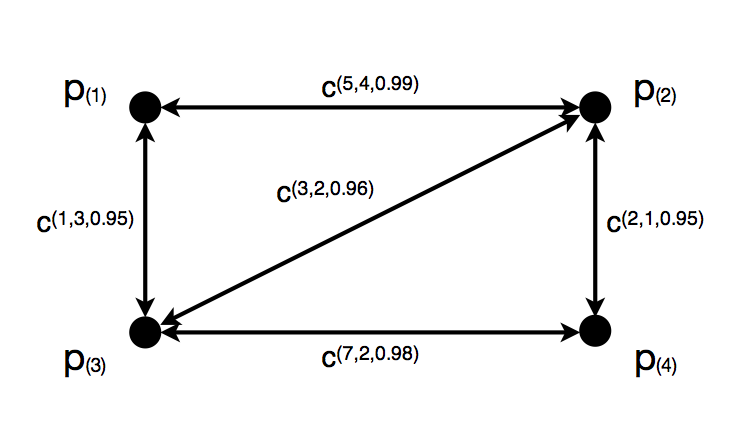
\includegraphics[width=10cm]{figure-8-plus.png}\end{center}

\noindent Entry $\prescript{2}{}{p_{21}} \in \mathbf{P}_2$ describes all satisfactory multi-weighted paths of length $2$ from vertex $2$ to vertex $1$, entry $\prescript{2}{}{p_{34}} \in \mathbf{P}_2$ describes all satisfactory multi-weighted paths of length $2$ from vertex $3$ to vertex $4$, and so on.
\end{example}

\newpage

\begin{prop}
Left-multiplying the $n$-by-$n$ cost-path matrix $\mathbf{M}$ by its corresponding $n$-by-$n$ matrix $\mathbf{P}_k$, where $\mathbf{P}_k = \mathbf{D} \times \mathbf{M} \times \mathbf{M} \times \ldots \times \mathbf{M}$ with $\mathbf{M}$ appearing $k$ times, results in an $n$-by-$n$ matrix $\mathbf{P}_{k+1} = \mathbf{P}_k \mathbf{M}$ whose entry $\prescript{k+1}{}{p_{ij}}$ in row $i$ and column $j$ lists exactly all satisfactory paths of length $k+1$ in $G$ from vertex $i$ to vertex $j$ along with the corresponding multi-weight for each of these paths.
\end{prop}

\begin{proof}
\hspace{1cm}

Let $k=1$ so that $\mathbf{P}_k = \mathbf{P}_1$ and $\mathbf{P_{k+1}} = \mathbf{P}_2$. The entry $\prescript{2}{}{p_{ij}}$ in row $i$ and column $j$ of the $n$-by-$n$ matrix $\mathbf{P}_2 = \mathbf{P}_1 \mathbf{M}$ lists exactly all satisfactory paths of length $2$ in $G$ from vertex $i$ to vertex $j$ along with the corresponding multi-weight for each of these paths.

Suppose that for some $k \in \N$, entry $\prescript{k}{}{p_{ij}} \in \mathbf{P}_k$ lists exactly all satisfactory paths of length $k$ in $G$ from vertex $i$ to vertex $j$ along with the corresponding multi-weight for each of these paths.

Let $\mathbf{P}_{k+1} = \mathbf{P}_k \mathbf{M}$. Each entry $\prescript{k+1}{}{p_{ij}} \in \mathbf{P}_{k+1}$ is given by $\prescript{k+1}{}{p_{ij}} = \sum_{r=1}^n \prescript{k}{}{p_{ir}} m_{rj} = \prescript{k}{}{p_{i1}}m_{1j} + \prescript{k}{}{p_{i2}}m_{2j} + \ldots + \prescript{k}{}{p_{in}}m_{nj} = p_{(i,\ldots,1)} \cdot p_{(j)} \sum_{h_{i1}=1}^{f_{i1}} c^{\vec{w}_{h_{i1}}} \sum_{h_{1j}=1}^{f_{1j}} c^{\vec{w}_{h_{1j}}} + p_{(i,\ldots,2)} \cdot p_{(j)} \sum_{h_{i2}=1}^{f_{i2}} c^{\vec{w}_{h_{i2}}} \allowbreak \sum_{h_{2j}=1}^{f_{2j}} c^{\vec{w}_{h_{2j}}} + \ldots + p_{(i,\ldots,n)} \cdot p_{(j)} \sum_{h_{in}=1}^{f_{in}} c^{\vec{w}_{h_{in}}} \sum_{h_{nj}=1}^{f_{nj}} c^{\vec{w}_{h_{nj}}}$.

For each $r \in \N : r \le n$, if $(i, \ldots, r, j)$ is a path in $G$ (i.e. $r$ is adjacent to $j$ with $(i, \ldots, r)$ being a path of length $k$ in $G$) with satisfactory multi-weights $\sum_{h_{ir}=1}^{f_{ir}} c^{\vec{w}_{h_{ir}}} \sum_{h_{rj}=1}^{f_{rj}} c^{\vec{w}_{h_{rj}}}$, then the terms $p_{(i,\ldots,r)} \cdot p_{(j)} \sum_{h_{ir}=1}^{f_{ir}} c^{\vec{w}_{h_{ir}}} \sum_{h_{rj}=1}^{f_{rj}} c^{\vec{w}_{h_{rj}}} = p_{(i,\ldots,r,j)} \sum_{h_{ir}=1}^{f_{ir}} c^{\vec{w}_{h_{ir}}} \sum_{h_{rj}=1}^{f_{rj}} c^{\vec{w}_{h_{rj}}}$, i.e. paths of length $k+1$ composed of all satisfactory paths $(i,\ldots,r)$ of length $k$ from vertex $i$ to some vertex $r$ and then directly to $j$ along with the corresponding multi-weight given by each multi-weight of a path $(i, \ldots, r)$ $\boxplus$ each multi-weight of an edge from $r$ to $j$.

Otherwise, if $\forall r \in \N : r \le n \implies p_{(i,\ldots,r)} \cdot p_{(j)} \sum_{h_{ir}=1}^{f_{ir}} c^{\vec{w}_{h_{ir}}} \sum_{h_{rj}=1}^{f_{rj}} c^{\vec{w}_{h_{rj}}} = 0$, then $\prescript{k+1}{}{p_{ij}} = 0$, indicating zero satisfactory paths of length $k+1$ in $G$ from vertex $i$ to vertex $j$.

Note that, for all other entries in $\mathbf{P}_{k+1}$, either the start vertex is not $i$ or the end vertex is not $j$, which means that no entry in $\mathbf{P}_{k+1}$ other than $\prescript{k+1}{}{p_{ij}}$ describes any paths from vertex $i$ to vertex $j$.

Further, suppose there exists a satisfactory path $(i, \ldots, r, j)$ of length $k+1$ in $G$ from vertex $i$ along some path $(i, \ldots, r)$ and finally to vertex $j$ that is not listed in entry $\prescript{k+1}{}{p_{ij}}$ (i.e. it does not appear in $\mathbf{P}_{k+1}$). Since the path from $i$ to $r$ is of length $k$, the it appears in $\mathbf{P}_k$ in entry $\prescript{k}{}{p_{ij}} $. Additionally, the cost-path element $c^{\vec{w}} p_{(j)}$ corresponding to the edge from $r$ to $j$ appears in entry $m_{rj}$ of $\mathbf{M}$. As a result, this satisfactory path $(i, \ldots, r, j)$ of length $k+1$ is accounted for in $\prescript{k+1}{}{p_{ij}} $, a contradiction of the supposition that this path is not listed in $\prescript{k+1}{}{p_{ij}}$. Thus, if there exists a satisfactory path of length $k+1$ in $G$ from a vertex $i$ along some path $(i, \ldots, r)$ of length $k$ and finally to vertex $j$, then it is listed in entry $\prescript{k+1}{}{p_{ij}}$. Since $r$ is arbitrary and entry $\prescript{k}{}{p_{ir}}$ describes all paths of length $k$ from $i$ to $r$, any satisfactory path of length $k+1$ from $i$ to $j$ is listed in entry $\prescript{k+1}{}{p_{ij}}$.

Therefore, entry $\prescript{k+1}{}{p_{ij}}$ in row $i$ and column $j$ lists all satisfactory paths of length $k+1$ in $G$ from vertex $i$ to vertex $j$ along with the corresponding multi-weight for each of these paths.
\end{proof}

\newpage

\begin{example}
Consider the matrix $\mathbf{P}_3 = \mathbf{P}_2 \mathbf{M}$.
$$
\mathbf{P}_3 = \begin{pmatrix}
0 & 0 & 0 & c^{(6,3,0.8664)} p_{(1,3,2,4)} \\
0 & 0 & 0 & 0 \\
0 & 0 & 0 & 0 \\
c^{(6,3,0.8664)} p_{(4,2,3,1)} & 0 & 0 & 0 \end{pmatrix}
$$
Consider the corresponding graph $G = \{V,E\}$.

\begin{center}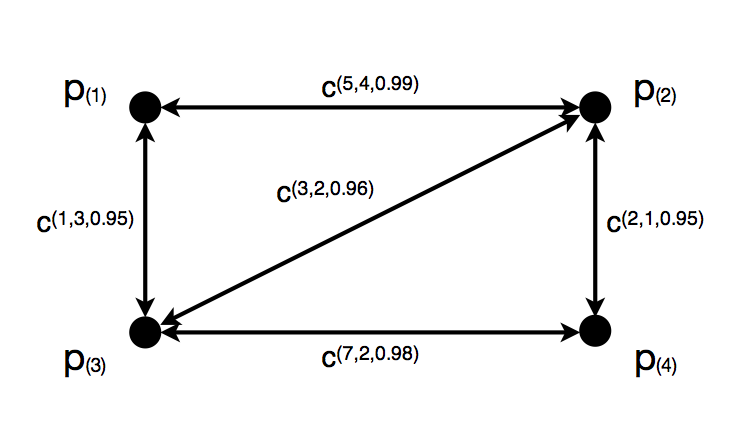
\includegraphics[width=10cm]{figure-8-plus.png}\end{center}

\noindent Entry $\prescript{3}{}{p_{41}}$ and entry  $\prescript{3}{}{p_{14}}$ in $\mathbf{P}_3$ describe the satisfactory paths of length $3$ in $G$.
\end{example}

\section{The Algorithm with an Example}

Given a graph $G = \{V,E\}$ of multi-weighted edges (for example, of additive, maximal, and multiplicative weight types, respectively), and a multi-constraint (for example, $(7, 4, 0.85)$), the algorithm finds the shortest satisfactory path(s) from some vertex $a \in V$ (for example, $a = 1$) to some vertex $z \in V$ (for example, $z = 4$).

\begin{center}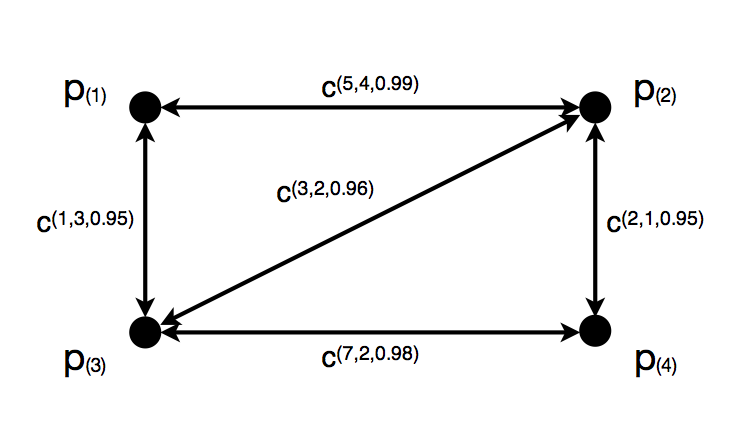
\includegraphics[width=10cm]{figure-8-plus.png}\end{center}

\step{0} \textbf{Generate} the graph's \textit{cost-path matrix}.
$$
\mathbf{M} = 
\begin{pmatrix}
0 & c^{(5,4,0.99)} p_{(2)} & c^{(1,3,0.95)} p_{(3)} & 0 \\
c^{(5,4,0.99)} p_{(1)} & 0 & c^{(3,2,0.96)} p_{(3)} & c^{(2,1,0.95)} p_{(4)} \\
c^{(1,3,0.95)} p_{(1)} & c^{(3,2,0.96)} p_{(2)} & 0 & c^{(7,2,0.98)} p_{(4)} \\
0 & c^{(2,1,0.95)} p_{(2)} & c^{(7,2,0.98)} p_{(3)} & 0 \end{pmatrix}
$$
\textbf{Calculate} the \textit{matrix $\mathbf{P}_1 = \mathbf{D}\mathbf{M}$}. \textbf{Select} a \textit{start vertex} $a$ (e.g. $1$) and an \textit{end vertex} $z$ (e.g. $4$). Calculating the matrices $\mathbf{P}_2$, $\mathbf{P}_3$, $\mathbf{P}_4$, and so on until the first matrix $\mathbf{P}_k$ with a nonzero entry $\prescript{k}{}{p_{az}}$ will reveal the solution. However, this approach actually solves a larger problem: finding all satisfactory paths of length $k$ in $G$. In order to reduce the number of calculations performed by the algorithm that do not directly relate to finding the shortest satisfactory path(s) from a particular start vertex to a particular end vertex, \textbf{select} only the \textit{$a^\text{th}$ row vector $\prescript{}{a}{\vec{P}_1}$ of $\mathbf{P}_1$}, which contains the entry $\prescript{1}{}{p}_{az}$. For example, $\prescript{}{1}{\vec{P}_1} = \begin{pmatrix} 0 & c^{(5,4,0.99)} p_{(1,2)} & c^{(1,3,0.95)} p_{(1,3)} & 0 \end{pmatrix}$. \textbf{If} the \textit{entry $\prescript{1}{}{p_{az}} \in \prescript{}{a}{\vec{P}_1}$} \textbf{is} \textit{nonzero}, \textbf{then} the algorithm \textbf{return}s \textit{entry $\prescript{1}{}{p_{az}}$} because it is the solution. \textbf{If} the \textit{$a^\text{th}$ row vector $\prescript{}{a}{\vec{P}_1}$} \textbf{is} the \textit{zero vector}, e.g. $\begin{pmatrix} 0 & 0 & 0 & 0 \end{pmatrix}$, \textbf{then} the algorithm \textbf{terminate}s because there is no solution.

\hspace{1cm}

\step{k : $k \in \N$} \textbf{Calculate} the \textit{row vector $\prescript{}{a}{\vec{P}_{k+1}} = \prescript{}{a}{\vec{P}_k} \mathbf{M}$}. For example, $\prescript{}{1}{\vec{P}_{2}} = $
$$
\begin{pmatrix} 0 & c^{(5,4,0.99)} p_{(1,2)} & c^{(1,3,0.95)} p_{(1,3)} & 0 \end{pmatrix}
\begin{pmatrix}
0 & c^{(5,4,0.99)} p_{(2)} & c^{(1,3,0.95)} p_{(3)} & 0 \\
c^{(5,4,0.99)} p_{(1)} & 0 & c^{(3,2,0.96)} p_{(3)} & c^{(2,1,0.95)} p_{(4)} \\
c^{(1,3,0.95)} p_{(1)} & c^{(3,2,0.96)} p_{(2)} & 0 & c^{(7,2,0.98)} p_{(4)} \\
0 & c^{(2,1,0.95)} p_{(2)} & c^{(7,2,0.98)} p_{(3)} & 0 \end{pmatrix}
$$
$$
= \begin{pmatrix} 0 & c^{(4,3,0.912)} p_{(1,3,2)} & 0 & 0 \end{pmatrix}
$$
\textbf{If} the \textit{entry $\prescript{k+1}{}{p_{az}} \in \prescript{}{a}{\vec{P}_{k+1}}$} \textbf{is} \textit{nonzero}, \textbf{then} the algorithm \textbf{return}s \textit{entry $\prescript{k+1}{}{p_{az}}$} because it is the solution. \textbf{If} the \textit{row vector $\prescript{}{a}{\vec{P}_{k+1}}$} \textbf{is} the \textit{zero vector}, \textbf{then} the algorithm \textbf{terminate}s because there is no solution. \textbf{Jump} to \step{k+1}.

\hspace{1cm}

\noindent In the example, the algorithm returns the solution $c^{(6,3,0.8664)} p_{(1,3,2,4)}$ in Step 2.
$$
\prescript{}{1}{\vec{P}_{3}} = \begin{pmatrix} 0 & c^{(4,3,0.912)} p_{(1,3,2)} & 0 & 0 \end{pmatrix}
\begin{pmatrix}
0 & c^{(5,4,0.99)} p_{(2)} & c^{(1,3,0.95)} p_{(3)} & 0 \\
c^{(5,4,0.99)} p_{(1)} & 0 & c^{(3,2,0.96)} p_{(3)} & c^{(2,1,0.95)} p_{(4)} \\
c^{(1,3,0.95)} p_{(1)} & c^{(3,2,0.96)} p_{(2)} & 0 & c^{(7,2,0.98)} p_{(4)} \\
0 & c^{(2,1,0.95)} p_{(2)} & c^{(7,2,0.98)} p_{(3)} & 0 \end{pmatrix}
$$
$$
= \begin{pmatrix} 0 & 0 & 0 & c^{(6,3,0.8664)} p_{(1,3,2,4)} \end{pmatrix}
$$
Since entry $\prescript{3}{}{p_{14}} \in \prescript{}{1}{\vec{P}_{3}}$ is nonzero, then $c^{(6,3,0.8664)} p_{(1,3,2,4)}$ is the solution.

\hspace{1cm}

Once the algorithm has returned the solution to the multi-constrained path problem, the optimal path may be selected in order to solve the multi-constrained optimal path problem. In this example, the solution to the multi-constrained optimal path problem is $c^{(6,3,0.8664)} p_{(1,3,2,4)}$.

A graph may be a good candidate for analysis with this algorithm if it reduces the number of calculations that the algorithm must perform in order to return the solution. For example, a graph in which each vertex is adjacent to an average of four other vertices and where the multi-weighted edges are multi-constrainted such that paths become unsatisfactory after an average path length of three would reduce the number of calculations that the algorithm must perform in order to return the solution.

On the other hand, graphs in which each vertex is adjacent to many other vertices or where the multi-weighted edges are multi-constrained such that paths rarely become unsatisfactory would require that the algorithm perform a large number of calculations in order to return the solution.

\newpage

\section{References}

\hspace{1cm}

\noindent Brualdi, R. (2004). \emph{Introductory Combinatorics, Fourth Edition}. Upper Saddle

River, NJ: Pearson Prentice Hall.\\

\noindent Fraleigh, J. (2003). \emph{A First Course in Abstract Algebra, Seventh Edition}. Boston, MA:

Addison Wesley.\\

\noindent Golan, J. (1999). \emph{Semirings and their Applications}. Norwell, MA: Kluwer Academic

Publishers.\\

\noindent Kahng, A. (1995). \emph{On Optimal Interconnections for VLSI}. Norwell, MA: Kluwer Academic

Publishers. \\

\noindent Meyer, C. (2000). \emph{Matrix Analysis and Applied Linear Algebra}. Philadelphia, PA: Society

for Industrial and Applied Mathematics. \\

\noindent Rosen, K. (2007). \emph{Discrete Mathematics and Its Applications, Sixth Edition}. St. Louis, MO:

McGraw Hill Higher Education. \\

\noindent Schott, R., and S. Staples. (2012). \emph{Operator Calculus on Generalized Zeon Algebras: Theory}

\emph{and Application to Multi-Constrained Path Problems}.

\verb+http://www.loria.fr/~schott/staceyQoS12.pdf+. \\

\noindent Staples, S. (2008). \emph{A new adjacency matrix for finite graphs}. Advances in Applied Clifford

Algebras. \\

\noindent Tucker, A. (2012). \emph{Applied Combinatorics, Sixth Edition}. Hoboken, NJ: Wiley. \\

\end{document}